\documentclass[tikz,border=10pt]{standalone}
\usepackage{tikz}
\usetikzlibrary{shapes,arrows,positioning,shadows,fit,backgrounds}

\begin{document}

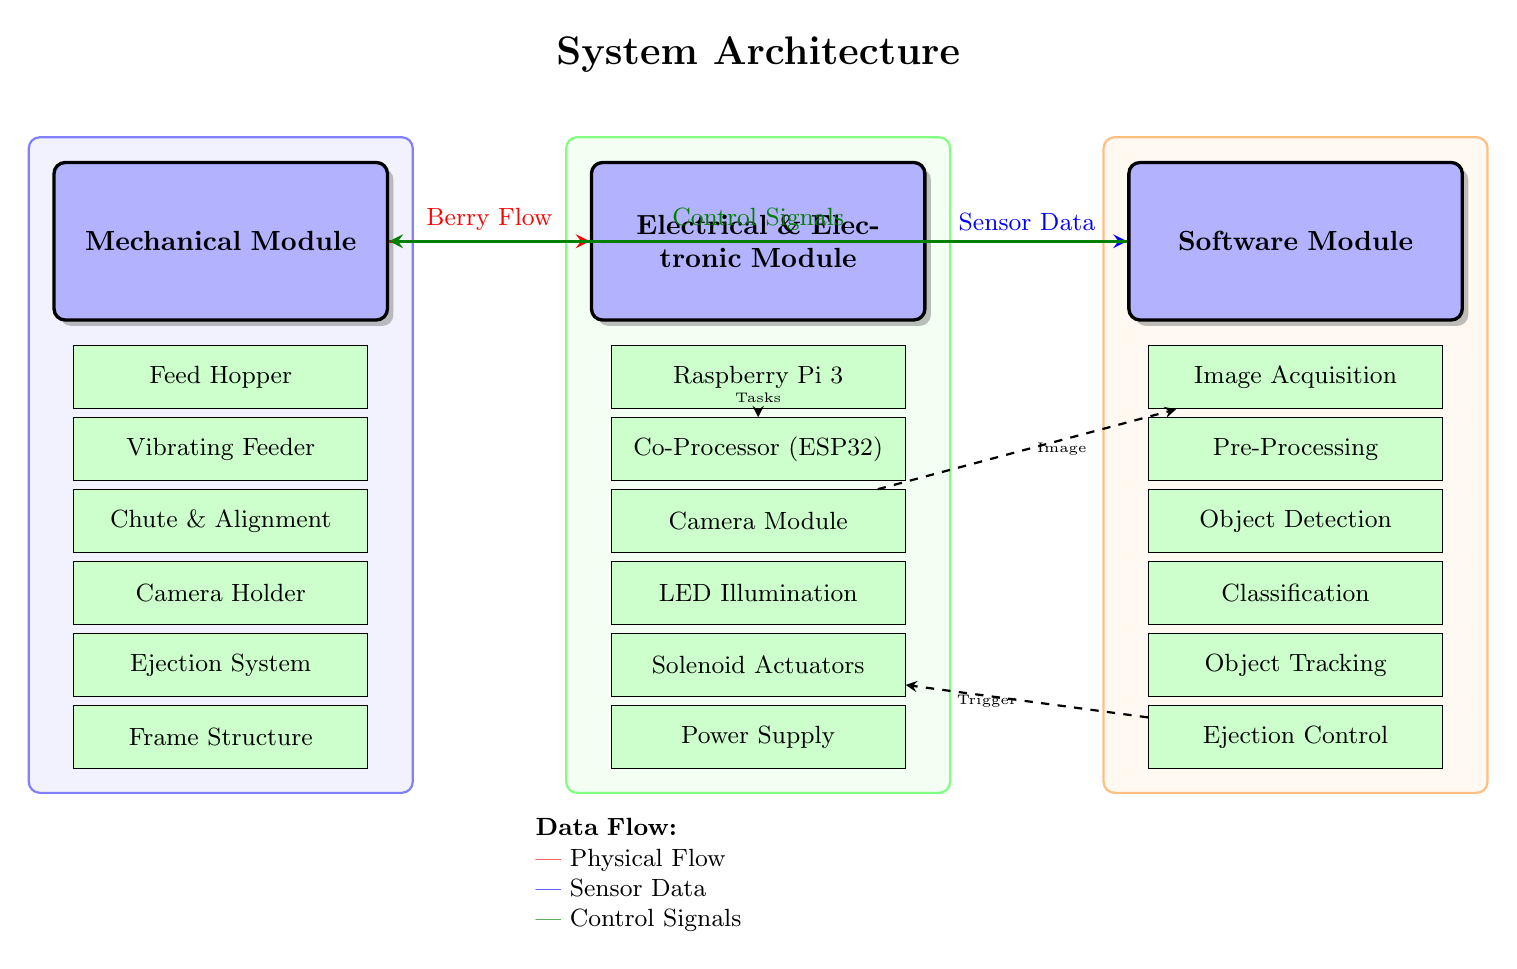
\begin{tikzpicture}[
    node distance=1.5cm,
    module/.style={rectangle, draw, fill=blue!30, text width=4cm, text centered, rounded corners, minimum height=2cm, drop shadow, very thick},
    component/.style={rectangle, draw, fill=green!20, text width=3.5cm, text centered, minimum height=0.8cm, font=\small},
    subcomp/.style={rectangle, draw, fill=yellow!20, text width=3cm, text centered, minimum height=0.6cm, font=\footnotesize},
    arrow/.style={thick,->,>=stealth},
    title/.style={font=\bfseries\Large}
]

% Title
\node[title] (title) {System Architecture};

% Three main modules
\node[module, below left=1cm and 2cm of title] (mechanical) {\textbf{Mechanical Module}};
\node[module, below=1cm of title] (electrical) {\textbf{Electrical \& Electronic Module}};
\node[module, below right=1cm and 2cm of title] (software) {\textbf{Software Module}};

% Mechanical components
\node[component, below=0.3cm of mechanical] (m1) {Feed Hopper};
\node[component, below=0.1cm of m1] (m2) {Vibrating Feeder};
\node[component, below=0.1cm of m2] (m3) {Chute \& Alignment};
\node[component, below=0.1cm of m3] (m4) {Camera Holder};
\node[component, below=0.1cm of m4] (m5) {Ejection System};
\node[component, below=0.1cm of m5] (m6) {Frame Structure};

% Electrical components
\node[component, below=0.3cm of electrical] (e1) {Raspberry Pi 3};
\node[component, below=0.1cm of e1] (e2) {Co-Processor (ESP32)};
\node[component, below=0.1cm of e2] (e3) {Camera Module};
\node[component, below=0.1cm of e3] (e4) {LED Illumination};
\node[component, below=0.1cm of e4] (e5) {Solenoid Actuators};
\node[component, below=0.1cm of e5] (e6) {Power Supply};

% Software components
\node[component, below=0.3cm of software] (s1) {Image Acquisition};
\node[component, below=0.1cm of s1] (s2) {Pre-Processing};
\node[component, below=0.1cm of s2] (s3) {Object Detection};
\node[component, below=0.1cm of s3] (s4) {Classification};
\node[component, below=0.1cm of s4] (s5) {Object Tracking};
\node[component, below=0.1cm of s5] (s6) {Ejection Control};

% Connections between modules
\draw[arrow, red, very thick] (mechanical) -- node[above, sloped, font=\small] {Berry Flow} (electrical);
\draw[arrow, blue, very thick] (electrical) -- node[above, sloped, font=\small] {Sensor Data} (software);
\draw[arrow, green!50!black, very thick] (software) -- node[above, sloped, font=\small] {Control Signals} (mechanical);

% Data flow arrows
\draw[arrow, dashed] (e3) -- node[right, font=\tiny] {Image} (s1);
\draw[arrow, dashed] (s6) -- node[left, font=\tiny] {Trigger} (e5);
\draw[arrow, dashed] (e1) -- node[above, font=\tiny] {Tasks} (e2);

% Background boxes
\begin{scope}[on background layer]
    \node[fit=(mechanical)(m6), fill=blue!5, draw=blue!50, thick, rounded corners, inner sep=0.3cm] {};
    \node[fit=(electrical)(e6), fill=green!5, draw=green!50, thick, rounded corners, inner sep=0.3cm] {};
    \node[fit=(software)(s6), fill=orange!5, draw=orange!50, thick, rounded corners, inner sep=0.3cm] {};
\end{scope}

% Legend
\node[below=0.5cm of m6, xshift=6cm, font=\small, text width=4cm] (legend) {
    \textbf{Data Flow:}\\
    {\color{red}—} Physical Flow\\
    {\color{blue}—} Sensor Data\\
    {\color{green!50!black}—} Control Signals
};

\end{tikzpicture}

\end{document}
